% -*- TeX-master: "main.tex" -*-

\begin{appendices}
\chapter{Glossary and Abbreviations}
\begin{multicols}{2}
\label{ch:glossary}
\begin{description}[leftmargin=0pt]
  \item[API]{Application Programming Interface, i.e., in
      case of an extension API, the functions and classes (names, arguments,
      etc.) an extension can implement.}
  \item[add-on]{A synonym for \emph{extension}.}
  \item[backend]{The software library doing the ``heavy lifting'' in
      qutebrowser, such as doing network requests or drawing website content.}
  \item[CI]{Continuous integration, i.e., running automated tests or other
      checks with every change.}
  \item[CSS]{Cascading Style Sheets, used to define styling/appearance of web pages.}
  \item[decorator] A \emph{Python} decorator allows annotating/wrapping a
    function. See section \ref{sec:langfeatures}.
  \item[DOM]{Document Object Model, the \emph{API} to access a HTML document as
      a tree structure.}
  \item[extension]{Code using an \emph{API} in order to extend the functionality
      of an existing project.}
  \item[GUI]{Graphical User Interface.}
  \item[HSR]{The Hochschule für Technik (University of Applied Sciences) in
      Rapperswil, Switzerland.}
  \item[HTML]{HyperText Markup Language, the language used to structure web
      pages.}
  \item[IDE]{Integrated Development Environment -- a software application
      providing tools (such as a source editor) for development.}
  \item[IFS]{The Institute for Software at \emph{HSR}.}
  \item[JavaScript]{The programming language used for interactive web sites.}
  \item[plugin]{In most contexts, the same as an \emph{extension}. Note that
      qutebrowser initially used \emph{plugin API} to refer to its extension
      API. However, this should be avoided, as ``plugin'' is too ambiguous in
      the context of web browsers: A plugin usually refers to software using the
      deprecated NPAPI (Netscape Plugin API) or PPAPI (Pepper Plugin API)
      technologies, such as Adobe Flash.}
  \item[Python]{The programming language used to write qutebrowser.}
  \item[PyQt]{A software library which allows to use \emph{Qt} from \emph{Python}.}
  \item[Qt]{The \emph{GUI} library used by qutebrowser.}
  \item[QtWebEngine]{The \emph{backend} used by default in qutebrowser, based on
      the Chromium project (like the Chrome web browser).}
  \item[QtWebKit]{One of two possible \emph{backends} qutebrowser can use.
      QtWebKit is the older backend, which is not used by default anymore, but is
      still supported.}
  \item[SA]{Studienarbeit (student research project).}
  \item[slot] A slot is the method or function connected to a \emph{signal} in
    \emph{Qt}. See section \ref{sec:langfeatures}.
  \item[signal] A signal is a \emph{Qt} feature which lets objects communicate
    with each other. See section \ref{sec:langfeatures}.
  \item[W3C]{World Wide Web Consortium, the standards body for web-related
      technologies such as HTML.}
\end{description}
\end{multicols}

\chapter{API documentation}
\label{ch:sphinx}
The API documentation on the following pages has been generated from Python
docstrings in the API implementation. Sphinx 1.8.2 was used.

{\let\clearpage\relax\chapter{Task description / Aufgabenstellung}}
The original task description for this project (written in German) can be found on page \pageref{ch:aufgabenstellung}ff.

\includepdf[pages={5-15,17-18},trim=0 2cm 0 1.8cm,clip,pagecommand=,offset=0 1cm]{./img/sphinx.pdf}
\label{ch:aufgabenstellung}
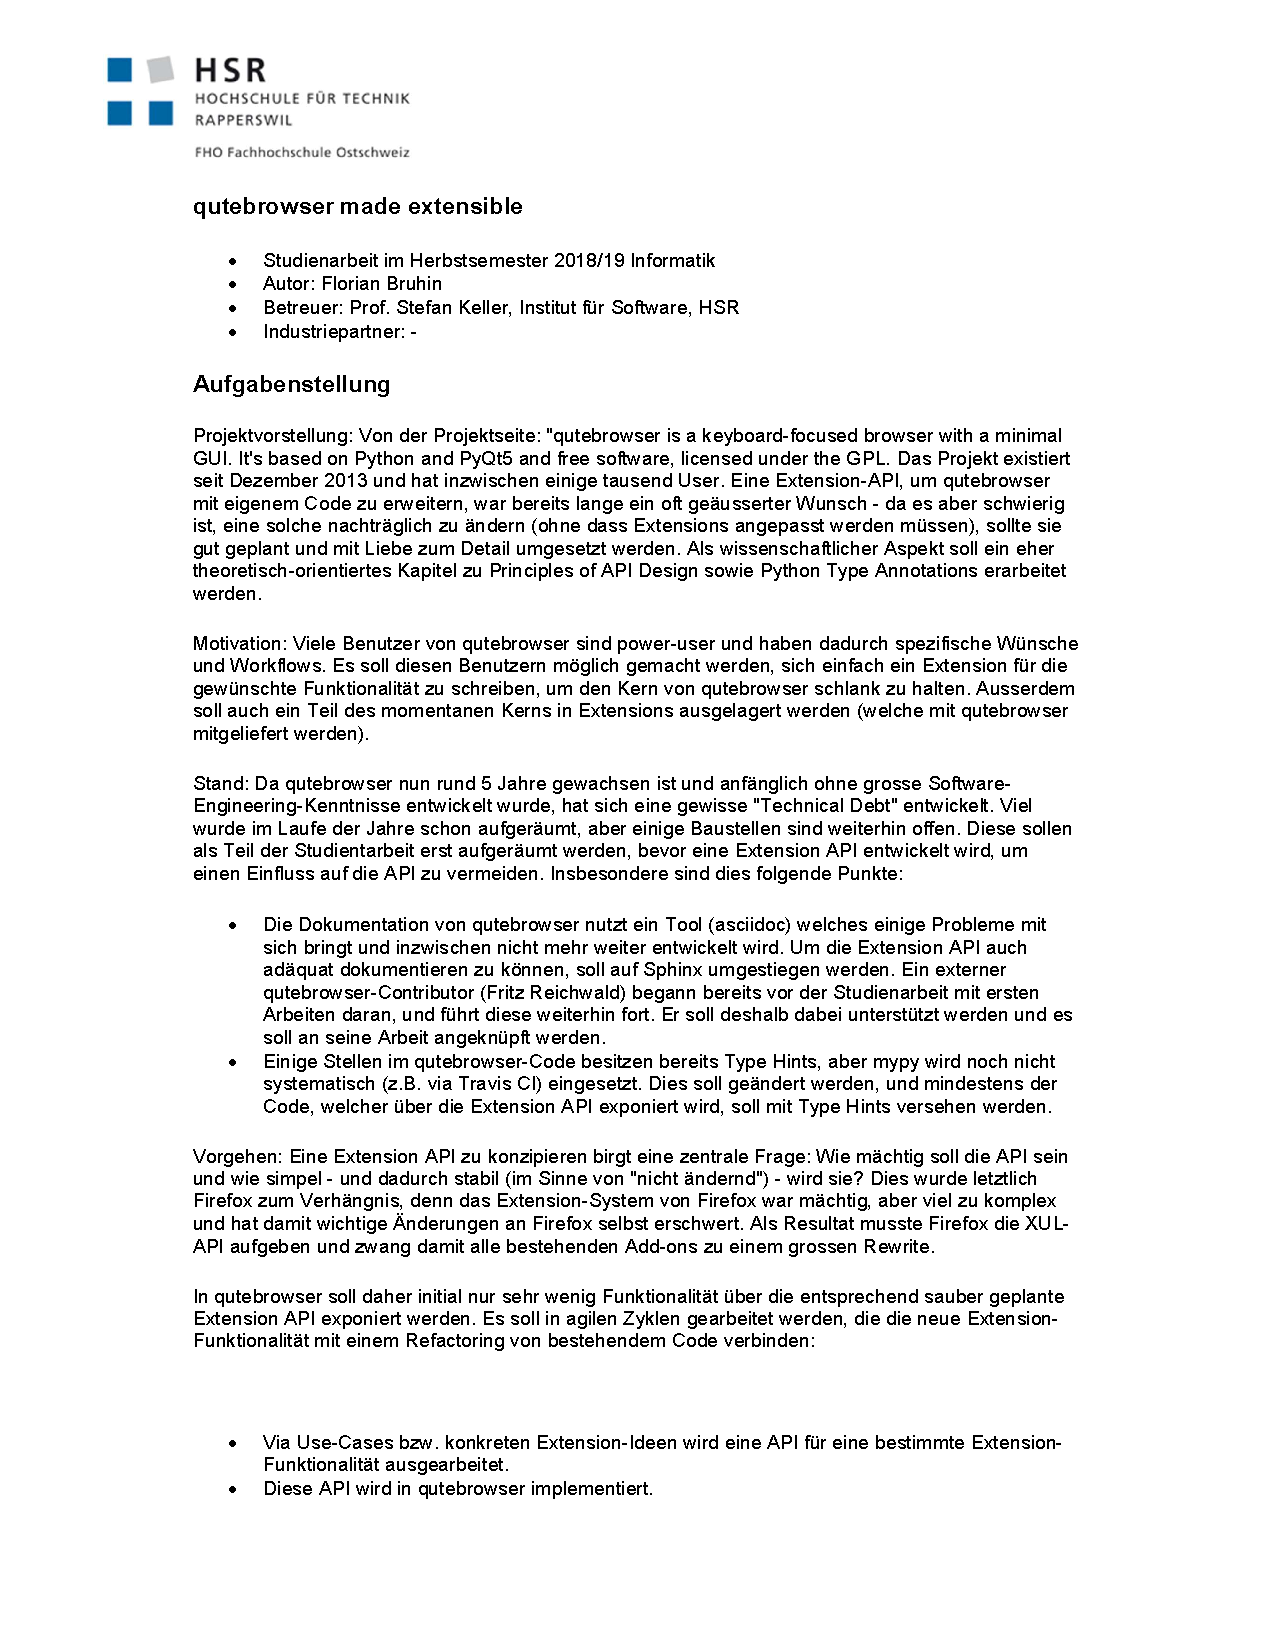
\includepdf[pages=-,pagecommand=]{./img/SA_Bruhin_Aufgabenstellung_v2.pdf}

\chapter{Urheber- und Nutzungsrechte}
Die Urheber- und Nutzungsrechte an der Software dieser Studierendenarbeit (nachfolgend ‚Arbeit’ genannt) sind im entsprechenden Software-Repository geregelt. Die Urheber- und Nutzungsrechte aller anderen Artefakte der Arbeit sind wie folgt geregelt: Die
Schutzrechte und das Know-how an den in diesem Rahmen geschaffenen Gütern (ausser Software, vgl. oben), stehen sowohl dem Rechtsträger der HSR Hochschule für Technik Rapperswil, dem für die Arbeit verantwortlichen Professoren, den allfällig beteiligten
Projektpartnern, sowie den Verfassern der Arbeit resp. Entwickler der in diesem Rahmen geschaffenen Güter zu. Die genannten Parteien übertragen sich gegenseitig nicht exklusiv, jedoch unentgeltlich, weltweit, sachlich und zeitlich unbeschränkt die
jeweiligen Schutzrechte und das Know-how an der Arbeit und an der in diesem Rahmen geschaffenen Güter, einschliesslich dem Recht zur Weiterübertragung, ab. Entsprechend steht es jeder Partei zu, sämtliche Schutzrechte an der Arbeit resp. an der in diesem
Rahmen geschaffenen Güter beliebig weltweit, zeitlich und sachlich unbeschränkt zu verwerten. Darunter fällt namentlich aber nicht abschliessend das Recht zur Lizenzierung in jeder Art, Umfang und Form, das Recht zur Bearbeitung und damit zur Nutzung als
Grundlage eines neuen schutzfähigen Guts. Die Parteien erklären sich gegenseitig den Verzicht auf Namensnennung bei der Verwertung der Schutzrechte und des Know-how durch eine oder mehrere Parteien gemeinsam und stimmen namentlich zu, dass jede Partei
allein unter ihrem eigenem Namen die Schutzrechte resp. das Know-how verwertet. Die vorliegende gegenseitige unentgeltliche Übertragung der Schutzrechte resp. des Know-how bezieht sich auch auf Verwertungsarten, welche heute noch nicht bekannt sind.



\chapter{Test log}
\label{ch:testlog}
\begin{minted}{text}
========================== test session starts ==========================
platform linux -- Python 3.7.1, pytest-4.0.1, py-1.7.0, pluggy-0.8.0
cachedir: .tox/py37/.pytest_cache
PyQt5 5.11.3 -- Qt runtime 5.12.0 -- Qt compiled 5.12.0
benchmark: 3.1.1 (defaults: [...])
hypothesis profile 'default' -> [...]
rootdir: /home/florian/proj/qutebrowser/git, inifile: pytest.ini
plugins: xvfb-1.1.0, travis-fold-1.3.0, rerunfailures-5.0, repeat-0.7.0,
  qt-3.2.1, mock-1.10.0, instafail-0.4.0, faulthandler-1.5.0, cov-2.6.0,
  benchmark-3.1.1, bdd-3.0.0, hypothesis-3.82.5
collected 195 items

tests/unit/api/test_cmdutils.py ..........................................
                                ...................
tests/unit/components/test_adblock.py ..............................
tests/unit/components/test_misccommands.py .....
tests/unit/extensions/test_loader.py ............
tests/unit/browser/webengine/test_webenginetab.py .....
tests/end2end/features/test_caret_bdd.py ...........
tests/end2end/features/test_scroll_bdd.py ..................s.............
                                          ...................
tests/end2end/features/test_zoom_bdd.py ...............x....


--------------- benchmark: 1 tests ---------------
Name (time in us)             Min      Max  Median
--------------------------------------------------
test_adblock_benchmark     3.3040  40.3980  3.4670
--------------------------------------------------

Legend:
  Outliers: 1 Standard Deviation from Mean; 1.5 IQR (InterQuartile Range)
            from 1st Quartile and 3rd Quartile.
  OPS: Operations Per Second, computed as 1 / Mean
=========== 193 passed, 1 skipped, 1 xfailed in 44.72 seconds ===========
\end{minted}

Tests marked with \emph{s}/\emph{skipped} were skipped because of
platform/environment differences. Tests marked with \emph{x}/\emph{xfailed} were
expected to fail due to known bugs.

Note only the subset of tests relevant to this project was ran.

\renewcommand{\bibname}{\chapter{Literature and Sources}\vspace{-1em}}
{\let\clearpage\relax\printbibliography}
\end{appendices}
